\section{A fixed state versus a growing cache at long horizon}
\label{sec:horizon}

\begin{figure}[t]
\centering
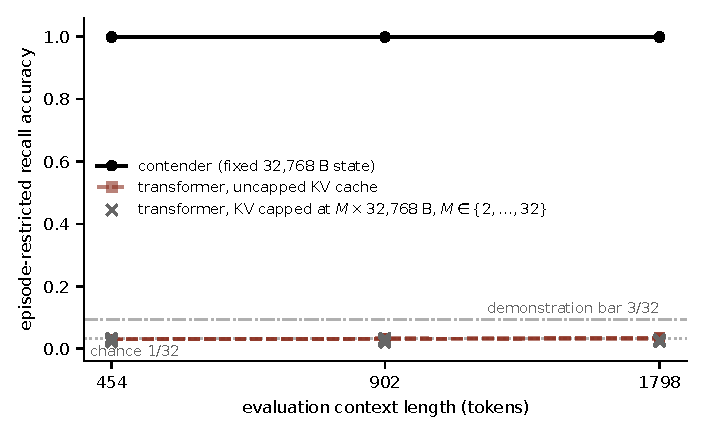
\includegraphics[width=0.86\linewidth]{figures/fig1_horizon.pdf}
\caption{Episode-restricted recall accuracy versus evaluation context
length (log scale) on the primary cell. Each episode's 224-token binding
span is embedded in filler continuation out to 454, 902, and 1{,}798
tokens. The matrix fast-weight model (three seeds, solid) holds
$\geq 0.998$ at every horizon with its state fixed at 32{,}768 bytes. The
transformer reads chance at every horizon, both uncapped (dashed) and
under sink-plus-FIFO KV caps at $M \times 32{,}768$ bytes for
$M \in \{2, \ldots, 32\}$ (crosses; $M{=}1$ is excluded from the walk
because its 8-token cap sits below the query length and is reported
descriptively in Table~\ref{tab:capped}). Reference lines mark chance
($1/32$) and the pre-registered demonstration bar ($3/32$).}
\label{fig:horizon}
\end{figure}

The constant-memory question is whether the recall of
Section~\ref{sec:recall} survives when the bound episode sits inside a
much longer context, with the fast-weight state's byte size unchanged. We
re-evaluate the same frozen checkpoints with each episode embedded in
filler continuation at three horizons: 454, 902, and 1{,}798 tokens, that
is, two, four, and eight times the binding span plus the
query. % <!-- evidence: C3 -->

\textbf{The fixed state does not decay.} The contender reads 0.9995,
0.9983, and 0.9990 (per seed) at \emph{every} horizon; the three curves in
Figure~\ref{fig:horizon} are flat to the third decimal from 454 to 1{,}798
tokens. % <!-- evidence: C3 -->
The state occupies 32{,}768 bytes at every point on the
curve. % <!-- evidence: C10 -->

\textbf{No cache budget rescues the baseline.} The uncapped transformer
reads 0.029 to 0.036 across seeds and horizons; % <!-- evidence: C4 -->
capped at every budget $M \times 32{,}768$ bytes for
$M \in \{2, \ldots, 32\}$ it reads 0.020 to 0.033, at or below its own
uncapped reading everywhere. % <!-- evidence: C4 -->
Per the frozen no-recall rule, these differences are chance-level
orderings. Two registered hypotheses die here at once. A larger cache
does not eventually hold the bindings: $M{=}32$ grants the cache more
bytes than the episode needs and the reading does not move. Forced
locality, which might have \emph{helped} by concentrating attention on
recent tokens, does not either; every capped reading sits at or below
uncapped.

\textbf{What is not claimed.} The registered degenerate-baseline clause
fires on this data exactly as written: the uncapped baseline itself fails
the demonstration bar at the primary cell (readings 0.0271 to 0.0293),
% <!-- evidence: C4 -->
so every cap is trivially cleared and the per-$M$ walk cannot certify a
memory-multiplier tier. Although each of the five eligible per-$M$ paired
gaps is individually clean (interval lower bounds all $\geq 0.9586$ at the
902-token decision horizon), % <!-- evidence: C4 -->
we quote no ``the fast-weight model matches at $M\times$ less memory''
figure, because there is no competent baseline reading to anchor the
ratio. The registered outcome is the sentence used throughout this paper:
baseline non-competitive at matched params/tokens. The two informative
facts are the contender's flat horizon curve at constant bytes and the
failure of every cap to change the baseline. Table~\ref{tab:capped} in the
appendix lists the full grid.
